% Options for packages loaded elsewhere
\PassOptionsToPackage{unicode}{hyperref}
\PassOptionsToPackage{hyphens}{url}
%
\documentclass[
]{article}
\usepackage{amsmath,amssymb}
\usepackage{lmodern}
\usepackage{iftex}
\ifPDFTeX
  \usepackage[T1]{fontenc}
  \usepackage[utf8]{inputenc}
  \usepackage{textcomp} % provide euro and other symbols
\else % if luatex or xetex
  \usepackage{unicode-math}
  \defaultfontfeatures{Scale=MatchLowercase}
  \defaultfontfeatures[\rmfamily]{Ligatures=TeX,Scale=1}
\fi
% Use upquote if available, for straight quotes in verbatim environments
\IfFileExists{upquote.sty}{\usepackage{upquote}}{}
\IfFileExists{microtype.sty}{% use microtype if available
  \usepackage[]{microtype}
  \UseMicrotypeSet[protrusion]{basicmath} % disable protrusion for tt fonts
}{}
\makeatletter
\@ifundefined{KOMAClassName}{% if non-KOMA class
  \IfFileExists{parskip.sty}{%
    \usepackage{parskip}
  }{% else
    \setlength{\parindent}{0pt}
    \setlength{\parskip}{6pt plus 2pt minus 1pt}}
}{% if KOMA class
  \KOMAoptions{parskip=half}}
\makeatother
\usepackage{xcolor}
\usepackage[margin=1in]{geometry}
\usepackage{color}
\usepackage{fancyvrb}
\newcommand{\VerbBar}{|}
\newcommand{\VERB}{\Verb[commandchars=\\\{\}]}
\DefineVerbatimEnvironment{Highlighting}{Verbatim}{commandchars=\\\{\}}
% Add ',fontsize=\small' for more characters per line
\usepackage{framed}
\definecolor{shadecolor}{RGB}{248,248,248}
\newenvironment{Shaded}{\begin{snugshade}}{\end{snugshade}}
\newcommand{\AlertTok}[1]{\textcolor[rgb]{0.94,0.16,0.16}{#1}}
\newcommand{\AnnotationTok}[1]{\textcolor[rgb]{0.56,0.35,0.01}{\textbf{\textit{#1}}}}
\newcommand{\AttributeTok}[1]{\textcolor[rgb]{0.77,0.63,0.00}{#1}}
\newcommand{\BaseNTok}[1]{\textcolor[rgb]{0.00,0.00,0.81}{#1}}
\newcommand{\BuiltInTok}[1]{#1}
\newcommand{\CharTok}[1]{\textcolor[rgb]{0.31,0.60,0.02}{#1}}
\newcommand{\CommentTok}[1]{\textcolor[rgb]{0.56,0.35,0.01}{\textit{#1}}}
\newcommand{\CommentVarTok}[1]{\textcolor[rgb]{0.56,0.35,0.01}{\textbf{\textit{#1}}}}
\newcommand{\ConstantTok}[1]{\textcolor[rgb]{0.00,0.00,0.00}{#1}}
\newcommand{\ControlFlowTok}[1]{\textcolor[rgb]{0.13,0.29,0.53}{\textbf{#1}}}
\newcommand{\DataTypeTok}[1]{\textcolor[rgb]{0.13,0.29,0.53}{#1}}
\newcommand{\DecValTok}[1]{\textcolor[rgb]{0.00,0.00,0.81}{#1}}
\newcommand{\DocumentationTok}[1]{\textcolor[rgb]{0.56,0.35,0.01}{\textbf{\textit{#1}}}}
\newcommand{\ErrorTok}[1]{\textcolor[rgb]{0.64,0.00,0.00}{\textbf{#1}}}
\newcommand{\ExtensionTok}[1]{#1}
\newcommand{\FloatTok}[1]{\textcolor[rgb]{0.00,0.00,0.81}{#1}}
\newcommand{\FunctionTok}[1]{\textcolor[rgb]{0.00,0.00,0.00}{#1}}
\newcommand{\ImportTok}[1]{#1}
\newcommand{\InformationTok}[1]{\textcolor[rgb]{0.56,0.35,0.01}{\textbf{\textit{#1}}}}
\newcommand{\KeywordTok}[1]{\textcolor[rgb]{0.13,0.29,0.53}{\textbf{#1}}}
\newcommand{\NormalTok}[1]{#1}
\newcommand{\OperatorTok}[1]{\textcolor[rgb]{0.81,0.36,0.00}{\textbf{#1}}}
\newcommand{\OtherTok}[1]{\textcolor[rgb]{0.56,0.35,0.01}{#1}}
\newcommand{\PreprocessorTok}[1]{\textcolor[rgb]{0.56,0.35,0.01}{\textit{#1}}}
\newcommand{\RegionMarkerTok}[1]{#1}
\newcommand{\SpecialCharTok}[1]{\textcolor[rgb]{0.00,0.00,0.00}{#1}}
\newcommand{\SpecialStringTok}[1]{\textcolor[rgb]{0.31,0.60,0.02}{#1}}
\newcommand{\StringTok}[1]{\textcolor[rgb]{0.31,0.60,0.02}{#1}}
\newcommand{\VariableTok}[1]{\textcolor[rgb]{0.00,0.00,0.00}{#1}}
\newcommand{\VerbatimStringTok}[1]{\textcolor[rgb]{0.31,0.60,0.02}{#1}}
\newcommand{\WarningTok}[1]{\textcolor[rgb]{0.56,0.35,0.01}{\textbf{\textit{#1}}}}
\usepackage{graphicx}
\makeatletter
\def\maxwidth{\ifdim\Gin@nat@width>\linewidth\linewidth\else\Gin@nat@width\fi}
\def\maxheight{\ifdim\Gin@nat@height>\textheight\textheight\else\Gin@nat@height\fi}
\makeatother
% Scale images if necessary, so that they will not overflow the page
% margins by default, and it is still possible to overwrite the defaults
% using explicit options in \includegraphics[width, height, ...]{}
\setkeys{Gin}{width=\maxwidth,height=\maxheight,keepaspectratio}
% Set default figure placement to htbp
\makeatletter
\def\fps@figure{htbp}
\makeatother
\setlength{\emergencystretch}{3em} % prevent overfull lines
\providecommand{\tightlist}{%
  \setlength{\itemsep}{0pt}\setlength{\parskip}{0pt}}
\setcounter{secnumdepth}{-\maxdimen} % remove section numbering
\ifLuaTeX
  \usepackage{selnolig}  % disable illegal ligatures
\fi
\IfFileExists{bookmark.sty}{\usepackage{bookmark}}{\usepackage{hyperref}}
\IfFileExists{xurl.sty}{\usepackage{xurl}}{} % add URL line breaks if available
\urlstyle{same} % disable monospaced font for URLs
\hypersetup{
  pdftitle={WORKING EXAMPLE 4},
  pdfauthor={Itziar Irigoien, Patricia Mas-Bermejo, Sergi Papiol, Neus Barrantes-Vidal,; Araceli Rosa, and Concepción Arenas},
  hidelinks,
  pdfcreator={LaTeX via pandoc}}

\title{WORKING EXAMPLE 4}
\usepackage{etoolbox}
\makeatletter
\providecommand{\subtitle}[1]{% add subtitle to \maketitle
  \apptocmd{\@title}{\par {\large #1 \par}}{}{}
}
\makeatother
\subtitle{In: A guide to test association between Polygenic Risk Scores
and psychological and psychiatric traits: practical examples}
\author{Itziar Irigoien, Patricia Mas-Bermejo, Sergi Papiol, Neus
Barrantes-Vidal, \and Araceli Rosa, and Concepción Arenas}
\date{}

\begin{document}
\maketitle

\hypertarget{working-flow-and-code}{%
\subsection{Working flow and code}\label{working-flow-and-code}}

In this example we simulate 10 PRSs, and a binary trait, with sex,
clinical diagnosis (with 2 categories), age, and two Principal
Components as covariates.

\begin{itemize}
\tightlist
\item
  data reading
\end{itemize}

\begin{Shaded}
\begin{Highlighting}[]
\NormalTok{dat }\OtherTok{\textless{}{-}} \FunctionTok{read.table}\NormalTok{(}\StringTok{"WExample4.csv"}\NormalTok{, }\AttributeTok{header=}\ConstantTok{TRUE}\NormalTok{, }\AttributeTok{sep=}\StringTok{";"}\NormalTok{, }\AttributeTok{dec=}\StringTok{","}\NormalTok{)}
\FunctionTok{names}\NormalTok{(dat) }\CommentTok{\#}
\end{Highlighting}
\end{Shaded}

\begin{verbatim}
##  [1] "Sex"        "Diagnostic" "Age"        "Trait"      "PRS.1"     
##  [6] "PRS.2"      "PRS.3"      "PRS.4"      "PRS.5"      "PRS.6"     
## [11] "PRS.7"      "PRS.8"      "PRS.9"      "PRS.10"     "PC1"       
## [16] "PC2"
\end{verbatim}

\bigskip

\begin{itemize}
\tightlist
\item
  do not forget to declare the categorical variables as factors
\end{itemize}

\begin{Shaded}
\begin{Highlighting}[]
\NormalTok{dat}\SpecialCharTok{$}\NormalTok{Sex }\OtherTok{\textless{}{-}} \FunctionTok{as.factor}\NormalTok{(dat}\SpecialCharTok{$}\NormalTok{Sex)}
\NormalTok{dat}\SpecialCharTok{$}\NormalTok{Diagnostic }\OtherTok{\textless{}{-}} \FunctionTok{as.factor}\NormalTok{(dat}\SpecialCharTok{$}\NormalTok{Diagnostic)}
\NormalTok{dat}\SpecialCharTok{$}\NormalTok{Trait }\OtherTok{\textless{}{-}} \FunctionTok{as.factor}\NormalTok{(dat}\SpecialCharTok{$}\NormalTok{Trait)}
\end{Highlighting}
\end{Shaded}

\hypertarget{what-full-model-should-be-considered}{%
\subsection{1. What full model should be
considered?}\label{what-full-model-should-be-considered}}

First, given a particular PRS (named PRS.i), consider all the possible
full models:

\begin{itemize}
\tightlist
\item
  FM\(_{WI}\): log(p/1-p) versus PRS.i + Sex + Diagnostic + Age + PC1 +
  PC2
\item
  FM\(_{Sex}\): log(p/1-p) versus PRS.i + Sex + PRS.i ·Sex + Diagnostic
  + Age + PC1 + PC2
\item
  FM\(_{Diagnostic}\): log(p/1-p) versus PRS.i + Sex + Diagnostic +
  PRS.i · Diagnostic + Age + PC1 + PC2
\item
  FM\(_{Sex/Diagnostic}\): log(p/1-p) versus PRS.i + Sex + PRS.i · Sex +
  Diagnostic + PRS.i · Diagnostic + Age + PC1 + PC2
\end{itemize}

\hypertarget{how-to-make-a-prs-ranking-to-find-the-important-ones}{%
\subsection{2. How to make a PRS ranking to find the important
ones?}\label{how-to-make-a-prs-ranking-to-find-the-important-ones}}

As is described in the paper, for each model, calculate the Tjur's
coefficients of discrimination. If Nagelkerke's \(R^2\) is prefered, set
statistic=``PseudoR2'' in function orderBin(), and calculate their sum,
\(S\).

According to S, list the PRSs in decreasing order:

\begin{Shaded}
\begin{Highlighting}[]
\CommentTok{\# Order the PRSs}
\NormalTok{out }\OtherTok{\textless{}{-}} \FunctionTok{orderBin}\NormalTok{(dat, }\AttributeTok{yname=}\StringTok{"Trait"}\NormalTok{, }\AttributeTok{prsname =} \StringTok{"PRS."}\NormalTok{, }\AttributeTok{statistic =} \StringTok{"D"}\NormalTok{)}
\FunctionTok{head}\NormalTok{(out)}
\end{Highlighting}
\end{Shaded}

\begin{verbatim}
##          Model1    Model2    Model3    Model4       Sum
## PRS.7 0.1816453 0.1816453 0.2175212 0.2176745 0.7984862
## PRS.8 0.1657769 0.1657769 0.1921405 0.1999160 0.7236103
## PRS.1 0.1644174 0.1644174 0.1716650 0.1874602 0.6879599
## PRS.2 0.1648077 0.1648077 0.1710979 0.1799683 0.6806815
## PRS.3 0.1638651 0.1638651 0.1735185 0.1785984 0.6798472
## PRS.4 0.1581438 0.1581438 0.1715735 0.1741957 0.6620568
\end{verbatim}

\begin{Shaded}
\begin{Highlighting}[]
\NormalTok{mainfilename }\OtherTok{\textless{}{-}} \StringTok{"WExample4"}
\NormalTok{filename }\OtherTok{\textless{}{-}} \FunctionTok{paste0}\NormalTok{(mainfilename, }\StringTok{"\_Ordered\_PRS.csv"}\NormalTok{)}
\FunctionTok{write.csv2}\NormalTok{(out,}\AttributeTok{file=}\NormalTok{filename)}
\end{Highlighting}
\end{Shaded}

Plot the sum of coefficients of discrimination coefficients \(D\).
Lines: in blue the median; in black the mean.

\begin{Shaded}
\begin{Highlighting}[]
\NormalTok{out }\OtherTok{\textless{}{-}} \FunctionTok{data.frame}\NormalTok{(out) }
\NormalTok{n }\OtherTok{\textless{}{-}} \FunctionTok{dim}\NormalTok{(out)[}\DecValTok{1}\NormalTok{]}
\NormalTok{select }\OtherTok{\textless{}{-}} \FunctionTok{grep}\NormalTok{(}\StringTok{"Model"}\NormalTok{, }\FunctionTok{names}\NormalTok{(out), }\AttributeTok{value=}\ConstantTok{FALSE}\NormalTok{)}
\NormalTok{out}\SpecialCharTok{$}\NormalTok{effect }\OtherTok{\textless{}{-}}\NormalTok{ out}\SpecialCharTok{$}\NormalTok{Sum}
\NormalTok{sds }\OtherTok{\textless{}{-}} \FunctionTok{apply}\NormalTok{(out[, select], }\DecValTok{1}\NormalTok{, sd)}
\NormalTok{out}\SpecialCharTok{$}\NormalTok{lower }\OtherTok{\textless{}{-}}\NormalTok{ out}\SpecialCharTok{$}\NormalTok{effect }\SpecialCharTok{{-}}\NormalTok{ sds}
\NormalTok{out}\SpecialCharTok{$}\NormalTok{upper }\OtherTok{\textless{}{-}}\NormalTok{ out}\SpecialCharTok{$}\NormalTok{effect }\SpecialCharTok{+}\NormalTok{ sds}
\NormalTok{out}\SpecialCharTok{$}\NormalTok{rank }\OtherTok{\textless{}{-}}\NormalTok{ n}\SpecialCharTok{:}\DecValTok{1}


\FunctionTok{ggplot}\NormalTok{(}\AttributeTok{data=}\NormalTok{out, }\FunctionTok{aes}\NormalTok{(}\AttributeTok{y=}\NormalTok{rank, }\AttributeTok{x=}\NormalTok{effect, }\AttributeTok{xmin=}\NormalTok{lower, }\AttributeTok{xmax=}\NormalTok{upper)) }\SpecialCharTok{+}
  \FunctionTok{geom\_point}\NormalTok{() }\SpecialCharTok{+}
  \FunctionTok{geom\_errorbarh}\NormalTok{(}\AttributeTok{height=}\NormalTok{.}\DecValTok{1}\NormalTok{) }\SpecialCharTok{+}
  \FunctionTok{scale\_y\_continuous}\NormalTok{(}\AttributeTok{name=}\ConstantTok{NULL}\NormalTok{, }\AttributeTok{breaks=}\NormalTok{ n}\SpecialCharTok{:}\DecValTok{1}\NormalTok{, }\AttributeTok{labels=}\FunctionTok{row.names}\NormalTok{(out), }\AttributeTok{position=}\StringTok{"right"}\NormalTok{) }\SpecialCharTok{+}
  \FunctionTok{labs}\NormalTok{(}\AttributeTok{title=}\StringTok{\textquotesingle{}\textquotesingle{}}\NormalTok{, }\AttributeTok{x=}\StringTok{\textquotesingle{}Sum of D\textquotesingle{}}\NormalTok{, }\AttributeTok{y =} \StringTok{\textquotesingle{}PRS\textquotesingle{}}\NormalTok{) }\SpecialCharTok{+}
  \FunctionTok{geom\_vline}\NormalTok{(}\AttributeTok{xintercept=}\FunctionTok{mean}\NormalTok{(out}\SpecialCharTok{$}\NormalTok{effect), }\AttributeTok{color=}\StringTok{\textquotesingle{}black\textquotesingle{}}\NormalTok{, }\AttributeTok{linetype=}\StringTok{\textquotesingle{}dashed\textquotesingle{}}\NormalTok{) }\SpecialCharTok{+}
  \FunctionTok{geom\_vline}\NormalTok{(}\AttributeTok{xintercept=}\FunctionTok{median}\NormalTok{(out}\SpecialCharTok{$}\NormalTok{effect), }\AttributeTok{color=}\StringTok{\textquotesingle{}blue\textquotesingle{}}\NormalTok{, }\AttributeTok{linetype=}\StringTok{\textquotesingle{}dashed\textquotesingle{}}\NormalTok{) }\SpecialCharTok{+}
  \FunctionTok{theme\_minimal}\NormalTok{()}
\end{Highlighting}
\end{Shaded}

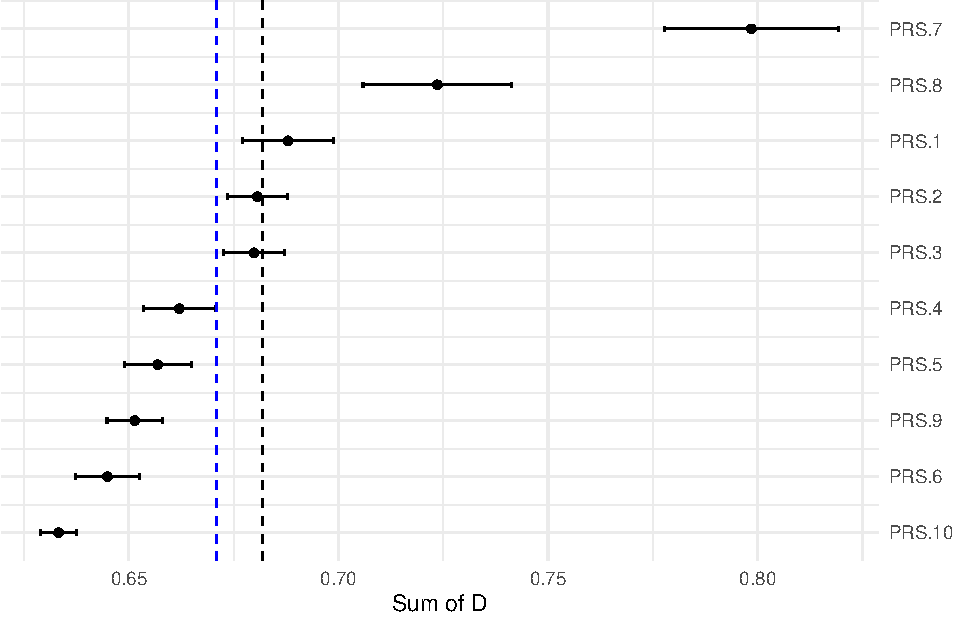
\includegraphics{WorkingExample4_code_files/figure-latex/unnamed-chunk-5-1.pdf}

According to the obtained results, first PRS.7 is selected to analyse
its association with the Trait.

\hypertarget{which-model-of-all-the-possible-ones-should-be-used}{%
\subsubsection{3. Which model, of all the possible ones, should be
used?}\label{which-model-of-all-the-possible-ones-should-be-used}}

The following figure represents the scatter plot separated by Sex and
Diagnostic groups.

\begin{Shaded}
\begin{Highlighting}[]
\CommentTok{\# First candidate PRS.7}
\CommentTok{\# Plot it}
\NormalTok{M }\OtherTok{\textless{}{-}} \FunctionTok{glm}\NormalTok{(Trait }\SpecialCharTok{\textasciitilde{}}\NormalTok{ PRS}\FloatTok{.7}\SpecialCharTok{*}\NormalTok{Sex }\SpecialCharTok{+}\NormalTok{ PRS}\FloatTok{.7}\SpecialCharTok{*}\NormalTok{Diagnostic }\SpecialCharTok{+}\NormalTok{ Age }\SpecialCharTok{+}\NormalTok{ PC1 }\SpecialCharTok{+}\NormalTok{ PC2, }\AttributeTok{data=}\NormalTok{dat, }\AttributeTok{family=}\FunctionTok{binomial}\NormalTok{())}
\NormalTok{pre }\OtherTok{\textless{}{-}}\NormalTok{ M}\SpecialCharTok{$}\NormalTok{fitted.values }\CommentTok{\#predict(M,type=\textquotesingle{}response\textquotesingle{})   }
\FunctionTok{ggplot}\NormalTok{(dat, }\FunctionTok{aes}\NormalTok{(}\AttributeTok{x=}\NormalTok{PRS}\FloatTok{.7}\NormalTok{, }\AttributeTok{y=}\FunctionTok{log}\NormalTok{(pre}\SpecialCharTok{/}\NormalTok{(pre}\SpecialCharTok{+}\DecValTok{1}\NormalTok{)))) }\SpecialCharTok{+}
  \FunctionTok{geom\_point}\NormalTok{(}\FunctionTok{aes}\NormalTok{(}\AttributeTok{color=}\NormalTok{Trait)) }\SpecialCharTok{+}
  \FunctionTok{geom\_smooth}\NormalTok{(}\AttributeTok{method=}\NormalTok{lm, }\AttributeTok{se=}\ConstantTok{FALSE}\NormalTok{)}\SpecialCharTok{+}
  \FunctionTok{facet\_grid}\NormalTok{(Sex }\SpecialCharTok{\textasciitilde{}}\NormalTok{ Diagnostic, }\AttributeTok{labeller=}\NormalTok{label\_both)}
\end{Highlighting}
\end{Shaded}

\begin{verbatim}
## `geom_smooth()` using formula = 'y ~ x'
\end{verbatim}

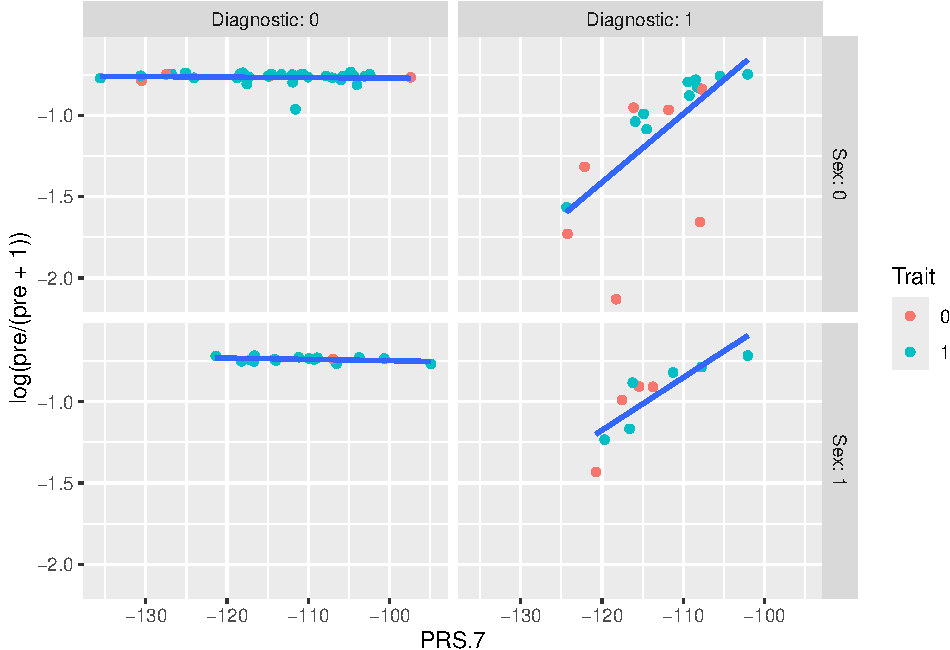
\includegraphics{WorkingExample4_code_files/figure-latex/unnamed-chunk-6-1.pdf}

\begin{Shaded}
\begin{Highlighting}[]
\CommentTok{\# Candidate FM Trait \textasciitilde{} PRS + Sex + Diagnostic + PRS*Diagnostic + C1 +C2}
\end{Highlighting}
\end{Shaded}

The plots suggest that the interaction between the PRS.7 and the
diagnostic is relevant. Thus, we set the full model candidate (FM):
\(log(p/1-p) \sim PRS + Sex + Diagnostic + PRS \cdot Diagnostic + Age + PC1 +PC2\).

\hypertarget{for-a-binary-trait-what-steps-should-be-followed-for-a-correct-analysis}{%
\subsubsection{5. For a binary trait, what steps should be followed for
a correct
analysis?}\label{for-a-binary-trait-what-steps-should-be-followed-for-a-correct-analysis}}

Check for overdispersion

\begin{Shaded}
\begin{Highlighting}[]
\CommentTok{\#model}
\NormalTok{FM }\OtherTok{\textless{}{-}} \FunctionTok{glm}\NormalTok{(Trait }\SpecialCharTok{\textasciitilde{}}\NormalTok{ Sex }\SpecialCharTok{+}\NormalTok{ PRS}\FloatTok{.7}\SpecialCharTok{*}\NormalTok{Diagnostic }\SpecialCharTok{+}\NormalTok{ Age }\SpecialCharTok{+}\NormalTok{ PC1 }\SpecialCharTok{+}\NormalTok{ PC2, }\AttributeTok{data=}\NormalTok{dat, }\AttributeTok{family=}\FunctionTok{binomial}\NormalTok{())}
\CommentTok{\#Residual Deviance}
\NormalTok{FM}\SpecialCharTok{$}\NormalTok{deviance}
\end{Highlighting}
\end{Shaded}

\begin{verbatim}
## [1] 67.46733
\end{verbatim}

\begin{Shaded}
\begin{Highlighting}[]
\CommentTok{\# Ratio }
\NormalTok{FM}\SpecialCharTok{$}\NormalTok{deviance}\SpecialCharTok{/}\NormalTok{FM}\SpecialCharTok{$}\NormalTok{df.residual}
\end{Highlighting}
\end{Shaded}

\begin{verbatim}
## [1] 0.92421
\end{verbatim}

Since this ratio is close to 1, there is not evidence of overdispersion.

\begin{Shaded}
\begin{Highlighting}[]
\CommentTok{\#With chi{-}squared test}
\NormalTok{FM.od }\OtherTok{\textless{}{-}} \FunctionTok{glm}\NormalTok{(Trait }\SpecialCharTok{\textasciitilde{}}\NormalTok{ Sex }\SpecialCharTok{+}\NormalTok{ PRS}\FloatTok{.7}\SpecialCharTok{*}\NormalTok{Diagnostic }\SpecialCharTok{+}\NormalTok{ Age }\SpecialCharTok{+}\NormalTok{ PC1 }\SpecialCharTok{+}\NormalTok{ PC2, }\AttributeTok{data=}\NormalTok{dat, }\AttributeTok{family=}\FunctionTok{quasibinomial}\NormalTok{())}
\FunctionTok{pchisq}\NormalTok{(}\FunctionTok{summary}\NormalTok{(FM.od)}\SpecialCharTok{$}\NormalTok{dispersion }\SpecialCharTok{*}\NormalTok{ FM}\SpecialCharTok{$}\NormalTok{df.residual,}
\NormalTok{       FM}\SpecialCharTok{$}\NormalTok{df.residual, }\AttributeTok{lower =} \ConstantTok{FALSE}\NormalTok{)}
\end{Highlighting}
\end{Shaded}

\begin{verbatim}
## [1] 0.3389642
\end{verbatim}

With this p-value = 0.3389, we conclude that there is not evidence of
overdispersion.

Based on the following table\ldots{}

\begin{Shaded}
\begin{Highlighting}[]
\FunctionTok{summary}\NormalTok{(FM)}
\end{Highlighting}
\end{Shaded}

\begin{verbatim}
## 
## Call:
## glm(formula = Trait ~ Sex + PRS.7 * Diagnostic + Age + PC1 + 
##     PC2, family = binomial(), data = dat)
## 
## Coefficients:
##                    Estimate Std. Error z value Pr(>|z|)  
## (Intercept)        1.953493   5.754567   0.339   0.7343  
## Sex1               0.445672   0.698490   0.638   0.5234  
## PRS.7              0.008372   0.051088   0.164   0.8698  
## Diagnostic1       16.714171  11.146266   1.500   0.1337  
## Age                0.043589   0.065843   0.662   0.5080  
## PC1               -5.565987   4.517987  -1.232   0.2180  
## PC2                3.784619   5.604881   0.675   0.4995  
## PRS.7:Diagnostic1  0.162405   0.097745   1.662   0.0966 .
## ---
## Signif. codes:  0 '***' 0.001 '**' 0.01 '*' 0.05 '.' 0.1 ' ' 1
## 
## (Dispersion parameter for binomial family taken to be 1)
## 
##     Null deviance: 83.234  on 80  degrees of freedom
## Residual deviance: 67.467  on 73  degrees of freedom
## AIC: 83.467
## 
## Number of Fisher Scoring iterations: 5
\end{verbatim}

\ldots the results show that PRS.7 is related with the log(p/1-p) in the
following way:

\begin{itemize}
\item
  \(\widehat{log(p/1-p)} = 1.953 + 0.008\times PRS.7 + 0.446\times Sex + 0.044\times Age - 5.566\times PC1 + 3.785\times PC2\),
  if Diagnostic = 0.
\item
  \(\widehat{log(p/1-p)} = (1.953+16.714) + (0.008+0.162)\times PRS.7 + 0.446\times Sex + 0.044\times Age - 5.566\times PC1 + 3.785\times PC2\),
  if Diagnostic = 1.
\end{itemize}

Check whether the respective PRS coefficients under each group are
significant or not.

\begin{Shaded}
\begin{Highlighting}[]
\FunctionTok{summary}\NormalTok{(}\FunctionTok{glht}\NormalTok{(FM, }\StringTok{"PRS.7 = 0"}\NormalTok{))}
\end{Highlighting}
\end{Shaded}

\begin{verbatim}
## 
##   Simultaneous Tests for General Linear Hypotheses
## 
## Fit: glm(formula = Trait ~ Sex + PRS.7 * Diagnostic + Age + PC1 + 
##     PC2, family = binomial(), data = dat)
## 
## Linear Hypotheses:
##            Estimate Std. Error z value Pr(>|z|)
## PRS.7 == 0 0.008372   0.051088   0.164     0.87
## (Adjusted p values reported -- single-step method)
\end{verbatim}

\begin{Shaded}
\begin{Highlighting}[]
\FunctionTok{summary}\NormalTok{(}\FunctionTok{glht}\NormalTok{(FM, }\StringTok{"PRS.7  + PRS.7:Diagnostic1 = 0"}\NormalTok{))}
\end{Highlighting}
\end{Shaded}

\begin{verbatim}
## 
##   Simultaneous Tests for General Linear Hypotheses
## 
## Fit: glm(formula = Trait ~ Sex + PRS.7 * Diagnostic + Age + PC1 + 
##     PC2, family = binomial(), data = dat)
## 
## Linear Hypotheses:
##                                Estimate Std. Error z value Pr(>|z|)  
## PRS.7 + PRS.7:Diagnostic1 == 0  0.17078    0.08476   2.015   0.0439 *
## ---
## Signif. codes:  0 '***' 0.001 '**' 0.01 '*' 0.05 '.' 0.1 ' ' 1
## (Adjusted p values reported -- single-step method)
\end{verbatim}

That means that for those with Diagnostic=0, it seems that the PRS.7 is
not related to the Trait with odds = \(\exp(0.0082) = 1.008\), but for
those with Diagnosis =1 the model indicates that the coefficient of
PRS.7 is 0.0082 + 0.162 = 0.1702, so the odds increase
\(\exp(0.1702) = 1.186\) for an incremental of one unit in PRS.7 with a
p-value=0.0439.

It is also possible to compute a permutation test to assess whether the
increase in the coefficient of determination \(D\) is significative.

\begin{Shaded}
\begin{Highlighting}[]
\CommentTok{\# Null model}
\NormalTok{NM }\OtherTok{\textless{}{-}} \FunctionTok{glm}\NormalTok{(Trait }\SpecialCharTok{\textasciitilde{}}\NormalTok{  Sex }\SpecialCharTok{+}\NormalTok{ Diagnostic }\SpecialCharTok{+}\NormalTok{ Age }\SpecialCharTok{+}\NormalTok{ PC1 }\SpecialCharTok{+}\NormalTok{ PC2, }\AttributeTok{data=}\NormalTok{dat, }\AttributeTok{family=}\FunctionTok{binomial}\NormalTok{() )}
\NormalTok{permtest }\OtherTok{\textless{}{-}} \FunctionTok{dD}\NormalTok{(NM, FM, }\AttributeTok{seed=}\DecValTok{1236}\NormalTok{)}
\NormalTok{permtest}
\end{Highlighting}
\end{Shaded}

\begin{verbatim}
## $dD
##          1 
## 0.07083991 
## 
## $pvalue
## [1] 0.09
\end{verbatim}

In this particular case, it can be seen that the coefficient of
discrimination of the FM model is 0.07 units bigger than the
corresponding to the \emph{Null Model} NM, but it is not statistically
significant.

\begin{itemize}
\tightlist
\item
  \textbf{Last step: We move to the next PRS.}
\end{itemize}

\end{document}
